% MoCoO Architecture Diagram — Standalone TikZ figure
% Compile: pdflatex -interaction=nonstopmode fig_architecture.tex
\documentclass[tikz,border=6pt]{standalone}
\usepackage[T1]{fontenc}
\usepackage[utf8]{inputenc}
\usepackage{amsmath,amssymb}
\usepackage{tikz}
\usetikzlibrary{
  arrows.meta,
  calc,
  fit,
  positioning,
  shapes.geometric,
  backgrounds,
}

% ── colour palette (IEEE-friendly, print-safe, colorblind-optimized) ──────────────────────────
\definecolor{cVAE}{RGB}{66,133,244}        % blue  – VAE (colorblind-safe)
\definecolor{cODE}{RGB}{230,120,20}        % orange – Neural ODE (enhanced saturation)
\definecolor{cMoCo}{RGB}{34,177,76}        % green  – MoCo (richer green)
\definecolor{cIB}{RGB}{155,89,182}         % purple – info bottleneck (improved luminance)
\definecolor{cLoss}{RGB}{180,60,60}        % muted red – losses
\definecolor{cInput}{RGB}{90,90,90}        % grey – I/O

% ── reusable styles ─────────────────────────────────────────────────────
\tikzset{
  basenode/.style={
    draw, rounded corners=2.5pt, minimum height=10.5mm,
    text width=23mm, align=center, font=\normalsize\sffamily,
    inner sep=2.5pt, line width=0.6pt,
  },
  vaebox/.style  ={basenode, fill=cVAE!10,  draw=cVAE!65},
  odebox/.style  ={basenode, fill=cODE!10,  draw=cODE!65},
  mocobox/.style ={basenode, fill=cMoCo!10, draw=cMoCo!65},
  ibbox/.style   ={basenode, fill=cIB!10,   draw=cIB!65},
  iobox/.style   ={basenode, fill=cInput!6, draw=cInput!45, text width=18mm},
  % queue with internal dividers
  queuebox/.style={
    draw=cMoCo!65, fill=cMoCo!7, rounded corners=1.5pt,
    minimum width=20mm, minimum height=8mm,
    font=\normalsize\sffamily, align=center,
    inner sep=2pt, line width=0.6pt,
    append after command={
      \pgfextra{
        \foreach \f in {0.2,0.4,0.6,0.8}{
          \draw[cMoCo!35, line width=0.35pt]
            ($(\tikzlastnode.north west)!\f!(\tikzlastnode.north east)$)
            -- ($(\tikzlastnode.south west)!\f!(\tikzlastnode.south east)$);
        }
      }
    },
  },
  % arrows
  dataflow/.style={
    -{Stealth[length=2.2mm,width=1.6mm]},
    line width=0.65pt, color=black!65,
  },
  lossflow/.style={
    -{Stealth[length=1.6mm,width=1.1mm]},
    line width=0.5pt, dashed, color=cLoss!75,
  },
  emaflow/.style={
    -{Stealth[length=1.6mm,width=1.1mm]},
    line width=0.5pt, densely dotted, color=cMoCo!70,
  },
  % labels
  annot/.style={font=\small\sffamily, text=black!65},
  lossannot/.style={font=\small\sffamily, text=cLoss!85},
}

\begin{document}
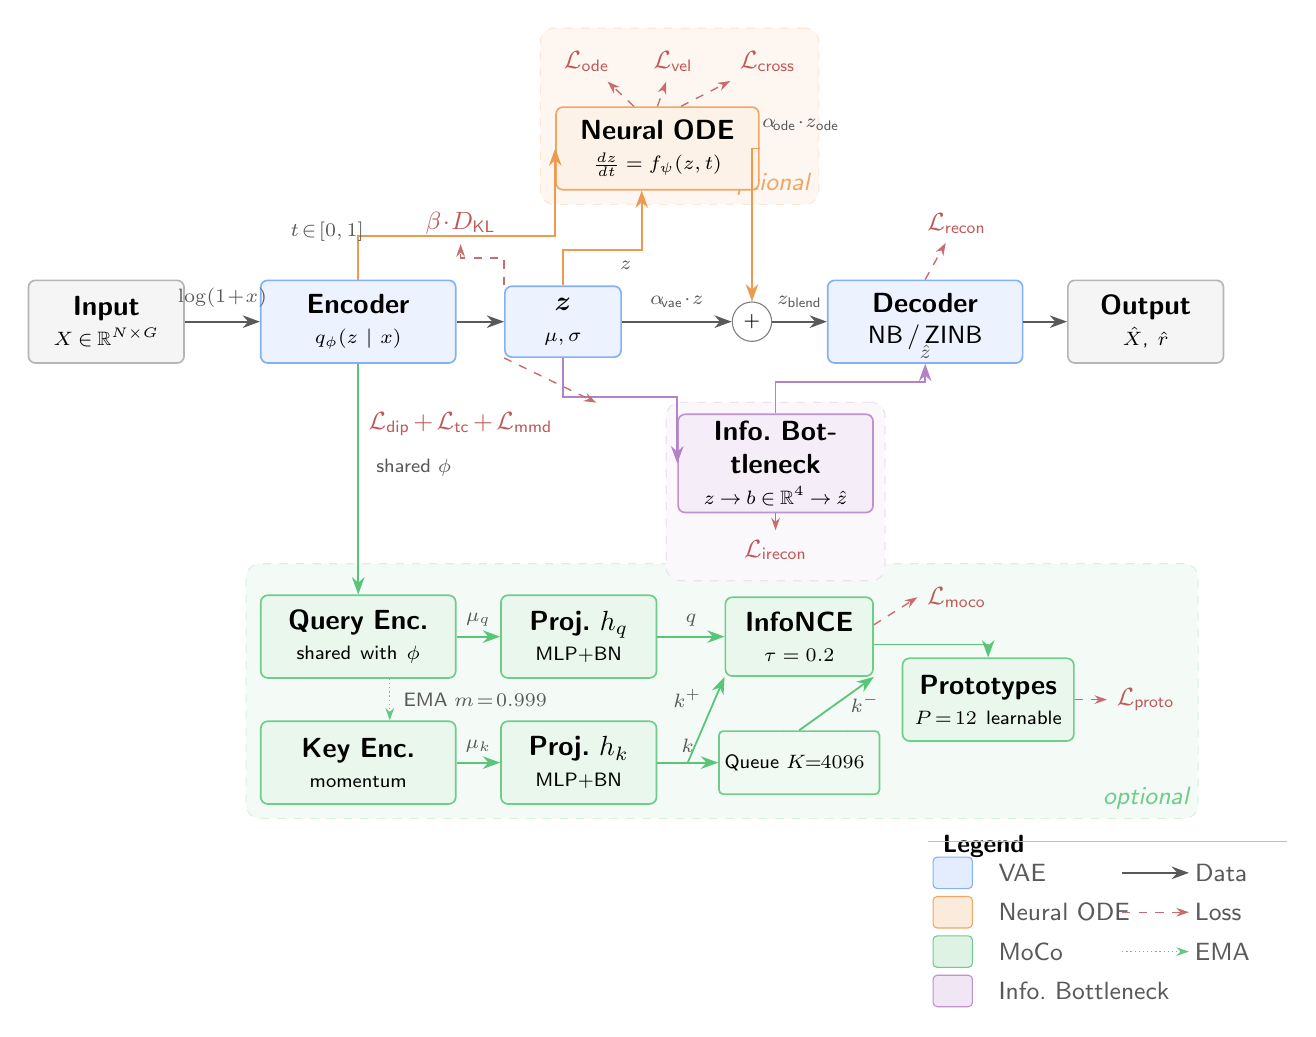
\begin{tikzpicture}

% =====================================================================
%  MAIN FLOW (y=0): Input -> Encoder -> z -> (+) -> Decoder -> Output
% =====================================================================

\node[iobox] (input) at (0,0) {
  \textbf{Input}\\[-1pt]
  {\scriptsize $X\!\in\!\mathbb{R}^{N\times G}$}
};

\node[vaebox] (enc) at (3.2,0) {
  \textbf{Encoder}\\[-1pt]
  {\scriptsize $q_\phi(z\!\mid\!x)$}
};

\node[vaebox, text width=13mm, minimum height=9mm] (z) at (5.8,0) {
  $\boldsymbol{z}$\\[-1pt]
  {\scriptsize $\mu,\sigma$}
};

% Blend circle (summation point)
\node[draw=black!50, fill=white, circle, inner sep=0pt,
      minimum size=5mm, font=\scriptsize\sffamily] (blend) at (8.2,0) {$+$};

\node[vaebox] (dec) at (10.4,0) {
  \textbf{Decoder}\\[-1pt]
  {\small NB\,/\,ZINB}
};

\node[iobox] (output) at (13.2,0) {
  \textbf{Output}\\[-1pt]
  {\scriptsize $\hat{X}$, $\hat{r}$}
};

% Main-flow arrows
\draw[dataflow] (input) -- node[annot, above, yshift=0.5mm]
  {\scriptsize $\log(1\!+\!x)$} (enc);
\draw[dataflow] (enc)   -- (z);
\draw[dataflow] (z)     -- node[annot, above, yshift=0.5mm]
  {\scriptsize $\alpha_{\!\text{vae}}\!\cdot\! z$} (blend);
\draw[dataflow] (blend) -- node[annot, above, yshift=0.5mm]
  {\scriptsize $z_{\text{blend}}$} (dec);
\draw[dataflow] (dec)   -- (output);

% =====================================================================
%  NEURAL ODE (above main flow, y ~ 2.2)
% =====================================================================

\node[odebox, text width=24mm] (ode) at (7.0,2.2) {
  \textbf{Neural ODE}\\[-1pt]
  {\scriptsize $\frac{dz}{dt}\!=\!f_\psi(z,t)$}
};

% Pseudotime from encoder hidden layer
\draw[dataflow, cODE!75]
  (enc.north) -- ++(0,0.55)
  node[annot, above left, xshift=2mm, yshift=-2mm] {\scriptsize $t\!\in\![0,1]$}
  -| (ode.west);

% z -> ODE
\draw[dataflow, cODE!75]
  (z.north) -- ++(0,0.45) -| node[annot, left, yshift=-2mm] {\scriptsize $z$}
  ([xshift=-2mm]ode.south);

% ODE -> blend (z_ode feeds blend circle)
\draw[dataflow, cODE!75]
  (ode.east) -| node[annot, right, yshift=3mm]
  {\scriptsize $\alpha_{\!\text{ode}}\!\cdot\! z_{\text{ode}}$} (blend.north);

% ODE losses
\node[lossannot] (odeloss) at (6.1,3.3) {$\mathcal{L}_{\text{ode}}$};
\node[lossannot] (velloss) at (7.2,3.3) {$\mathcal{L}_{\text{vel}}$};
\node[lossannot] (crossloss) at (8.4,3.3) {$\mathcal{L}_{\text{cross}}$};
\draw[lossflow] ([xshift=-3mm]ode.north) -- (odeloss);
\draw[lossflow] (ode.north) -- (velloss);
\draw[lossflow] ([xshift=3mm]ode.north) -- (crossloss);

% =====================================================================
%  INFORMATION BOTTLENECK (below blend/decoder area)
% =====================================================================

\node[ibbox, text width=23mm] (ib) at (8.5,-1.8) {
  \textbf{Info.\ Bottleneck}\\[-1pt]
  {\scriptsize $z\!\to\! b\!\in\!\mathbb{R}^4\!\to\!\hat{z}$}
};

% z -> IB (route right then down)
\draw[dataflow, cIB!75]
  (z.south) -- ++(0,-0.5) -| (ib.west);

% IB -> decoder (short upward connection)
\draw[dataflow, cIB!75]
  (ib.north) -- ++(0,0.4) -|
  node[annot, above, near end, yshift=0.5mm] {\scriptsize $\hat{z}$}
  (dec.south);

% IB loss
\node[lossannot] (ibloss) at (8.5,-2.9) {$\mathcal{L}_{\text{irecon}}$};
\draw[lossflow] (ib.south) -- (ibloss);

% =====================================================================
%  LOSSES near z and decoder
% =====================================================================

% KL divergence (above z, offset left to avoid ODE branch)
\node[lossannot] (klloss) at (4.5,1.25) {$\beta\!\cdot\! D_{\text{KL}}$};
\draw[lossflow] (z.north west) -- ++(0,0.35) -| (klloss);

% Reconstruction loss (above decoder)
\node[lossannot] (reconloss) at (10.8,1.25) {$\mathcal{L}_{\text{recon}}$};
\draw[lossflow] (dec.north) -- (reconloss);

% Disentanglement losses (between enc and z, below main flow)
\node[lossannot, text width=32mm, align=center] (disloss) at (4.5,-1.3) {
  {\small $\mathcal{L}_{\text{dip}}\!+\!\mathcal{L}_{\text{tc}}\!+\!\mathcal{L}_{\text{mmd}}$}
};
\draw[lossflow] (z.south west) -- (disloss.north east);

% =====================================================================
%  MOMENTUM CONTRAST (below, y ~ -4.0 to -5.6)
% =====================================================================

% Query encoder (shared weights with main encoder)
\node[mocobox, text width=23mm] (encq) at (3.2,-4.0) {
  \textbf{Query Enc.}\\[-1pt]
  {\scriptsize shared with $\phi$}
};

% Key encoder (EMA-updated copy)
\node[mocobox, text width=23mm] (enck) at (3.2,-5.6) {
  \textbf{Key Enc.}\\[-1pt]
  {\scriptsize momentum}
};

% Projection heads
\node[mocobox, text width=18mm] (projq) at (6.0,-4.0) {
  \textbf{Proj.\ $h_q$}\\[-1pt]
  {\scriptsize MLP+BN}
};
\node[mocobox, text width=18mm] (projk) at (6.0,-5.6) {
  \textbf{Proj.\ $h_k$}\\[-1pt]
  {\scriptsize MLP+BN}
};

% InfoNCE
\node[mocobox, text width=17mm, minimum height=10mm] (infonce) at (8.8,-4.0) {
  \textbf{InfoNCE}\\[-1pt]
  {\scriptsize $\tau\!=\!0.2$}
};

% Memory queue
\node[queuebox] (queue) at (8.8,-5.6) {
  {\scriptsize Queue $K\!\!=\!\!4096$}
};

% Prototypes
\node[mocobox, text width=20mm] (proto) at (11.2,-4.8) {
  \textbf{Prototypes}\\[-1pt]
  {\scriptsize $P\!=\!12$ learnable}
};

% --- MoCo internal arrows ---

% Encoder -> Query Enc (shared weights, straight down)
\draw[dataflow, cMoCo!75]
  (enc.south) -- (encq.north)
  node[annot, pos=0.45, right, xshift=1mm] {\scriptsize shared $\phi$};

% EMA update (query -> key, dotted)
\draw[emaflow] ([xshift=4mm]encq.south) --
  node[annot, right, xshift=0.5mm] {\scriptsize EMA $m\!=\!0.999$}
  ([xshift=4mm]enck.north);

% Query path: encq -> projq -> InfoNCE
\draw[dataflow, cMoCo!75] (encq) --
  node[annot, above] {\scriptsize $\mu_q$} (projq);
\draw[dataflow, cMoCo!75] (projq) --
  node[annot, above] {\scriptsize $q$} (infonce);

% Key path: enck -> projk -> queue
\draw[dataflow, cMoCo!75] (enck) --
  node[annot, above] {\scriptsize $\mu_k$} (projk);
\draw[dataflow, cMoCo!75] (projk) --
  node[annot, above] {\scriptsize $k$} (queue);

% Positive key: fork from k path, diagonal up-left to InfoNCE bottom-left
\coordinate (kfork) at ($(projk.east)!0.5!(queue.west)$);
\draw[dataflow, cMoCo!75]
  (kfork) -- node[annot, left, near end, xshift=-0.5mm] {\scriptsize $k^+$}
  (infonce.south west);

% Negative keys: queue -> InfoNCE (straight up, right side)
\draw[dataflow, cMoCo!75]
  (queue.north) --
  node[annot, right, xshift=0.5mm] {\scriptsize $k^-$}
  (infonce.south east);

% Projected features -> prototypes (from InfoNCE east, L-shaped right-down)
\draw[dataflow, cMoCo!75]
  ([yshift=-1mm]infonce.east) -| (proto.north);

% MoCo loss (to the right of InfoNCE, clean horizontal)
\node[lossannot] (mocoloss) at (10.8,-3.5) {$\mathcal{L}_{\text{moco}}$};
\draw[lossflow] ([yshift=1.5mm]infonce.east) -- (mocoloss.west);

% Prototype loss
\node[lossannot] (protoloss) at (13.2,-4.8) {$\mathcal{L}_{\text{proto}}$};
\draw[lossflow] (proto.east) -- (protoloss.west);

% =====================================================================
%  BACKGROUND REGIONS (shaded, dashed borders)
% =====================================================================
\begin{scope}[on background layer]
  % ODE region
  \node[fit=(ode)(odeloss)(crossloss),
        fill=cODE!6, draw=cODE!18, dashed, rounded corners=5pt,
        inner sep=5pt, label={[annot, anchor=south east, cODE!65,
        font=\small\sffamily\itshape]south east:optional}] {};

  % MoCo region
  \node[fit=(encq)(enck)(projq)(projk)(queue)(infonce)(proto)(protoloss)(mocoloss),
        fill=cMoCo!5, draw=cMoCo!18, dashed, rounded corners=5pt,
        inner sep=5pt, label={[annot, anchor=south east, cMoCo!65,
        font=\small\sffamily\itshape]south east:optional}] {};

  % IB region
  \node[fit=(ib)(ibloss),
        fill=cIB!4, draw=cIB!18, dashed, rounded corners=5pt,
        inner sep=4pt] {};
\end{scope}

% =====================================================================
%  LEGEND (bottom-right, enhanced two-column layout)
% =====================================================================
\begin{scope}[shift={(10.5,-6.4)}]
  \node[font=\small\sffamily\bfseries, anchor=north west] at (0,0) {Legend};
  \draw[black!25, line width=0.4pt] (-0.6mm,-2mm) -- (45mm,-2mm);

  % Colour patches (left column)
  \node[fill=cVAE!15, draw=cVAE!65, rounded corners=1.5pt,
        minimum width=5mm, minimum height=4mm, inner sep=0pt]
    (lv) at (2.5mm,-6mm) {};
  \node[annot, right=2mm of lv, anchor=west] {VAE};

  \node[fill=cODE!15, draw=cODE!65, rounded corners=1.5pt,
        minimum width=5mm, minimum height=4mm, inner sep=0pt]
    (lo) at (2.5mm,-11mm) {};
  \node[annot, right=2mm of lo, anchor=west] {Neural ODE};

  \node[fill=cMoCo!15, draw=cMoCo!65, rounded corners=1.5pt,
        minimum width=5mm, minimum height=4mm, inner sep=0pt]
    (lm) at (2.5mm,-16mm) {};
  \node[annot, right=2mm of lm, anchor=west] {MoCo};

  \node[fill=cIB!15, draw=cIB!65, rounded corners=1.5pt,
        minimum width=5mm, minimum height=4mm, inner sep=0pt]
    (li) at (2.5mm,-21mm) {};
  \node[annot, right=2mm of li, anchor=west] {Info.\ Bottleneck};

  % Arrow styles (right column)
  \draw[dataflow]  (24mm,-6mm)  -- ++(8.5mm,0)
    node[annot, right, xshift=-0.5mm] {Data};
  \draw[lossflow]  (24mm,-11mm)  -- ++(8.5mm,0)
    node[annot, right, xshift=-0.5mm] {Loss};
  \draw[emaflow]   (24mm,-16mm) -- ++(8.5mm,0)
    node[annot, right, xshift=-0.5mm] {EMA};
\end{scope}

\end{tikzpicture}
\end{document}
